
\documentclass[a4paper, twoside]{article}
\usepackage[backend=biber,style=ieee,sorting=none]{biblatex}
\usepackage{geometry}
\geometry{a4paper,total={170mm,250mm},left=20mm, top=20mm,}
\usepackage{enumerate}
\usepackage[shortlabels]{enumitem}
\usepackage{optidef}
\usepackage[normalem]{ulem}
\useunder{\uline}{\ul}{}
\addbibresource{mybibliography.bib}
\usepackage{datetime}
\usepackage{tableof}
\usepackage{amssymb}
\usepackage{algpseudocode}
\usepackage{multirow}
\usepackage{graphicx}
\usepackage{amsmath}
\usepackage{pdfpages}

\newdateformat{monthyeardate}{%
  \monthname[\THEMONTH], \THEYEAR}
\date{\monthyeardate\today}
%%%%%%%%%%%%%%%%%%%%%%%%%%%%%%%%%%%%%%%%%%%%%%%%%%%%%%%%%%%%%%%%%%%%%%%%%%%%%%%%%%%%%
%%%%%%%%%%%%%%%%%%%%%%%%%%%   Enter Your info here    %%%%%%%%%%%%%%%%%%%%%%%%%%%%%%%

\author{Benjamin Tollison}
\def\snum{Author}
\def\coursecode{AERO321}
\def\coursetitle{Dynamics of Aerospace Vehicles}
\def\assignname{Interim Report 2}

\title{Fall 23 Project}

%%%%%%%%%%%%%%%%%%%%%%%%%%%%%%%%%%%%%%%%%%%%%%%%%%%%%%%%%%%%%%%%%%%%%%%%%%%%%%%%%%%%%%



\begin{document}
\begin{titlepage}

\newcommand{\HRule}{\rule{\linewidth}{0.5mm}} % Defines a new command for the horizontal lines, change thickness here

%----------------------------------------------------------------------------------------
%	LOGO SECTION
%----------------------------------------------------------------------------------------
\centering

\includegraphics[width=8cm]{title/logo.png}\\[1cm] % Include a department/university logo - this will require the graphicx package
 
%----------------------------------------------------------------------------------------

\center % Center everything on the page

%----------------------------------------------------------------------------------------
%	HEADING SECTIONS
%----------------------------------------------------------------------------------------

\textsc{\LARGE \assignname}\\[1.5cm] %assignment name
\textsc{\Large \coursecode}\\[0.5cm] %Course code 
\textsc{\large \coursetitle}\\[0.5cm]  %Course title

%----------------------------------------------------------------------------------------
%	TITLE SECTION
%----------------------------------------------------------------------------------------
\makeatletter
\HRule \\[0.4cm]
{ \huge \bfseries \@title}\\[0.4cm] % Title of your document
\HRule \\[1.5cm]
 
%----------------------------------------------------------------------------------------
%	AUTHOR SECTION
%----------------------------------------------------------------------------------------

\begin{minipage}{0.4\textwidth}
\begin{flushleft} \large
\emph{Group Members}\\
\text{Jirina Bredberg}\\[1.2em]
\text{Ines Meyer}\\[1.2em]
\text{Kanishka Kamal}\\[1.2em]
\@author\\[1.2em] % Your name
\end{flushleft}
\end{minipage}
~
\begin{minipage}{0.4\textwidth}
\begin{flushright} \large
\emph{Tasks} \\
\text{Tables 1,2,5} \\[1.2em] 
\text{Tables 1,3,7} \\[1.2em] 
\text{Tables 3,4,6}\\[1.2em] 
\text{Author/Debugger,8} \\[1.2em] 
\end{flushright}
\end{minipage}\\[2cm]
\makeatother

%----------------------------------------------------------------------------------------
%	DATE SECTION
%----------------------------------------------------------------------------------------

{\large \today}\\[2cm] % Date, change the \today to a set date if you want to be precise

\vfill % Fill the rest of the page with whitespace

\end{titlepage}
\tableofcontents
\newpage
\section{Task 1a}
Determine the trim AoA, tail incidence angle, equilibrium thrust, and the normal force with the following system of equations in the body-axis system:
\[\sum{F_X} = 0 = T_0 - W\sin\alpha_0 + L_{WF}\sin\alpha_0-D_0\cos\alpha_0 + L_H\sin(\alpha_0-\epsilon)\]
\[\sum{F_Z}=0 = -F_{N_0} + W\cos\alpha_0 - L_{WF}\cos\alpha_0-D_0\sin\alpha_0 - L_H\cos(\alpha_0-\epsilon)\]
\begin{align*}
\sum{M_{cg}}= 0 = F_{N_0}(X_{cg}-X_{inlet}) - L_{WF}(X_{AC_{WF}}-X_{cg})\cos\alpha_0\\
- D_0(X_{AC_{WF}}-X_{cg})\sin\alpha_0 - L_{H}(X_{AC_{H}}-X_{cg})\cos(\alpha_0-\epsilon)
\end{align*}
A systematic approach to solving a system of equations involves breaking down the problem into manageable steps. 
Initially, one focuses on solving each equation by isolating the capitalized coefficients. 
This often requires employing linear approximations to better understand the behavior of each equation. 
The next step is to deconstruct the equations further, systematically breaking them down into simpler forms that are easier to solve. 
This iterative process allows for a methodical exploration of the system's intricacies, 
gradually unveiling solutions and facilitating a more comprehensive understanding of the relationships among the variables. 
Through this systematic method, one navigates the complexity of the system, step by step, until arriving at a point where the 
equations can be effectively solved.
\subsection{Determining \(L_{WF}\)}
It is stated that we can neglect the lift from the fuselage in the project assigment such that
\[L_{WF} \approx L_W = q_\infty S_W C_{L_W}\]
Find \(C_{L_W} \approx C_{L_{W0}} + C_{L_{\alpha,W}} \alpha_0\)\\
where \(C_{L_{W0}}=0\) due to symmetry, which leads to the problem that we need to now find \(C_{L_{\alpha,W}}\)

\subsection{Finding \(C_{L_{\alpha,W}}\)}
\begin{enumerate}
\item Find Taper ratio \(\lambda = \frac{2S_w}{bc_r}\)\\
\item Find SweepAngle of the LE: \(\Lambda_{LE} = \tan^{-1}\left(\tan{\Lambda_{c/4}} + \frac{1}{AR}\frac{1-\lambda}{1+\lambda}\right)\)\\
\item Find SweepAngle of the c/2: \(\Lambda_{c/2} = \tan^{-1}\left(\tan{\Lambda_{LE}} - \frac{2}{AR}\frac{1-\lambda}{1+\lambda}\right)\)\\
\item Find \(C_{l_\alpha} = \frac{2\pi}{\sqrt{1-M_\infty^2}}\)\\
\item Find beta/k constants: \(\beta = \sqrt{1-M^2}$, $k = \frac{C_{l_\alpha}}{2\pi}\)\\
\item plug into equation:
\end{enumerate}
\[C_{L_\alpha} = \frac{2\pi AR}{2+\sqrt{\frac{AR^2\beta^2}{k^2}\left(1+\frac{\tan^2{\Lambda_{c/2}}}{\beta^2}\right)+4}}\]

\subsection{Find \(q_\infty\)}
\[q_\infty = \frac{1}{2} \rho_\infty v_\infty^2\]\\
\begin{enumerate}
\item Get speed of sound from the tables: \(a = 296.5338[m/s]\)\\
\item Find \(v_\infty$ from $M = \frac{v_\infty}{a}\)\\
\item Get the \(\rho_\infty\) with isentropic equation
  \begin{enumerate}
  \item \(\frac{\rho_0}{\rho} = \left(1+\frac{\gamma-1}{2}M^2\right)^\frac{1}{\gamma-1}\)
  \item \(\rho_0 = 7.3654\cdot10^{-4} [sl/ft^3] = 0.3795971165326[kg/m^3]\)
  \end{enumerate}
\end{enumerate}
\[ \therefore L_{WF} = q_\infty S_W C_{L_{\alpha,W}} \alpha_0\]

\subsection{Finding \(D_0\)}
\[\rightarrow D_0 \equiv D(\alpha_0)\]
\[ D = q_\infty S_W C_D\]
\begin{enumerate}
\item Find $C_D$ from the given equation: $ C_D = 0.0145 + 0.1 C_{L_W}^2$
  \begin{enumerate}
  \item with $C_{L_W} = C_{L_{\alpha,W}}\alpha_0$
  \end{enumerate}
\end{enumerate}
\[\therefore D_0 = q_\infty S_W (0.0145 + 0.1C_{L_{\alpha,W}}^2 \alpha_0^2)\]

\subsection{Finding \(L_H\)}
\[ L_H = \eta_H \frac{S_H}{S_W} C_{L_H}\]
\subsection*{Finding \(C_{L_H}\)}
\[ C_{L_H} \equiv C_{L_H}(\alpha,\epsilon,i_H)\]
\begin{enumerate}
  
\item $\epsilon$ is also a function of $\alpha$
\item $C_{L_H} \approx C_{L_{H0}} + C_{L_{\alpha,H}}\alpha_H + C_{L_{i_H}} i_H | C_{L_{H0}} = 0,{symmetry}$
\item set $\alpha_H = \alpha_0 + i_H - \frac{d\epsilon}{d\alpha_W}\alpha_0$
\item- Find $C_{L_\alpha,H}$ with the same process as the wing
  \begin{enumerate}
  \item Find Taper ratio $\lambda = \frac{2S_w}{bc_r}$
  \item Find SweepAngle of the LE: $\Lambda_{LE} = \tan^{-1}\left(\tan{\Lambda_{c/4}} + \frac{1}{AR}\frac{1-\lambda}{1+\lambda}\right)$
  \item Find SweepAngle of the c/2: $\Lambda_{c/2} = \tan^{-1}\left(\tan{\Lambda_{LE}} - \frac{2}{AR}\frac{1-\lambda}{1+\lambda}\right)$
  \item Find $C_{l_\alpha} = \frac{2\pi}{\sqrt{1-M_\infty^2}}$
  \item Find Beta/k constants: $\beta = \sqrt{1-M^2}$, $k = \frac{C_{l_\alpha}}{2\pi}$
  \item plug into equation:
  \end{enumerate}
  \[C_{L_{\alpha,H}} = \frac{2\pi AR}{2+\sqrt{\frac{AR^2\beta^2}{k^2}\left(1+\frac{\tan^2{\Lambda_{c/2}}}{\beta^2}\right)+4}} \]
\item Find $C_{L_{i_H}}$ from the given equation: $C_{L_{i_H}} = C_{L_{\alpha,H}}\eta_H\frac{S_H}{S_W}$
\end{enumerate}
\[ \therefore L_H = \eta_H \frac{S_H}{S_W} C_{L_{\alpha,H}}\left(\alpha_0 + i_H - \frac{d\epsilon}{d\alpha_W}\alpha_0\right) + C_{L_{\alpha,H}}\eta_H\frac{S_H}{S_W} i_H \]

\subsection{Finding \(F_{N_0}\)}
Using the given equation
\[F_{N_0} = 2 q_\infty A_{inlet} \cos\alpha_0^2 \sin\alpha_0\]
\(A_{inlet}$ is given as 15 $ft^2$ or 1.39355 $m^2\)
\subsection{Finding \(\epsilon\)}
\(\epsilon\) estimated purely as a function of \(\alpha\)
\[\epsilon = \frac{d\epsilon}{d\alpha_W} (\alpha_W-\alpha_0)\]
where \(\alpha_0\) is 0 because it is a symmetrical airfoil
\[\therefore \epsilon  = \frac{d\epsilon}{d\alpha}\alpha_0 \]
Then with only 3 unknowns remaining of \(T_0,\alpha_0,i_H\), we used the SciPy fsolve function to solve the system of nonlinear equations.

\section{Task 1b}
Determine the most forward c.g. location from the tail incidence angle limit condition. \\
\subsection{Equations to consider}
\begin{equation}
CL(a, ih) = CL_{\alpha_{wf}} \cdot a + n_H \cdot CL_{\alpha_H} \cdot \left(a \cdot (1 - \delta_{e\delta a}) + ih\right) \cdot \frac{S_H}{S_W}
\end{equation}

\begin{equation}
CL_H(a, ih) = CL_{\alpha_H} \cdot \left(a \cdot (1 - \delta_{e\delta a}) + ih\right)
\end{equation}

\begin{equation}
CL_{wf}(a) = CL_{\alpha_{wf}} \cdot a
\end{equation}

\begin{equation}
CM(a, ih) = CL_{wf}(a) \cdot (X_{cg} - X_{ac_{wf}}) - n_H \cdot CL_H(a, ih) \cdot (X_{ac_H} - X_{cg}) \cdot \frac{S_H}{S_W}
\end{equation}
\begin{equation}
  CL_{\text{min}} = \frac{W}{q_{\text{inf}}\cdot S_{\text{W}}}
\end{equation}
\pagebreak
\subsection{Algorithm}
The method to find the forward most positon of the center of gravity uses the following algorithm: \\
\begin{enumerate}
    \item \textbf{Initialization:}
        \begin{itemize}
            \item Set the minimum coefficient of lift $CL_{\text{min}}$ based on aircraft weight ($W$), dynamic pressure ($q_{\text{inf}}$), and wing reference area ($S_{\text{W}}$).
            \item Generate an array $a$ with 1000 elements, ranging from -0.2 to 0.2.
        \end{itemize}
        
    \item \textbf{Iterative Process:}
        \begin{itemize}
            \item Iterate over a range of values for $i$ from 0 to 26.
            \item Initialize empty lists for $CL_{\text{list}}$ and $CM_{\text{list}}$.
            \item Calculate the midpoint ($xcg$) between $xcg_{\text{high}}$ and $xcg_{\text{low}}$.
            \item Set lower and upper bounds ($ilow$ and $iup$) for a pitch angle ($ih$) within a specified range.
            \item Calculate a guess for $ih$ ($guess_ih$) as the midpoint between $ilow$ and $iup$.
            \item Iterate over the range of $a$ values:
                \begin{itemize}
                    \item Calculate $CL$ and $CM$ for each $a$ and $ih$.
                    \item Append these values to $CL_{\text{list}}$ and $CM_{\text{list}}$.
                \end{itemize}
            \item Find the index ($l$) corresponding to the minimum value in $CM_{\text{list}}$.
            \item Calculate the angle of attack ($alpha$) and the guessed $CL$ value ($CL_{\text{guess}}$) based on the minimum $CM$.
            \item Adjust the bounds for $ih$ based on $CL_{\text{guess}}$ relative to $CL_{\text{min}}$.
            \item Adjust $xcg_{\text{high}}$ or $xcg_{\text{low}}$ based on the magnitude of $ih$ if it's less than or greater than 20 degrees.
        \end{itemize}
\end{enumerate}
\pagebreak

\section{Task 1 Tables}
\subsection*{Givens}
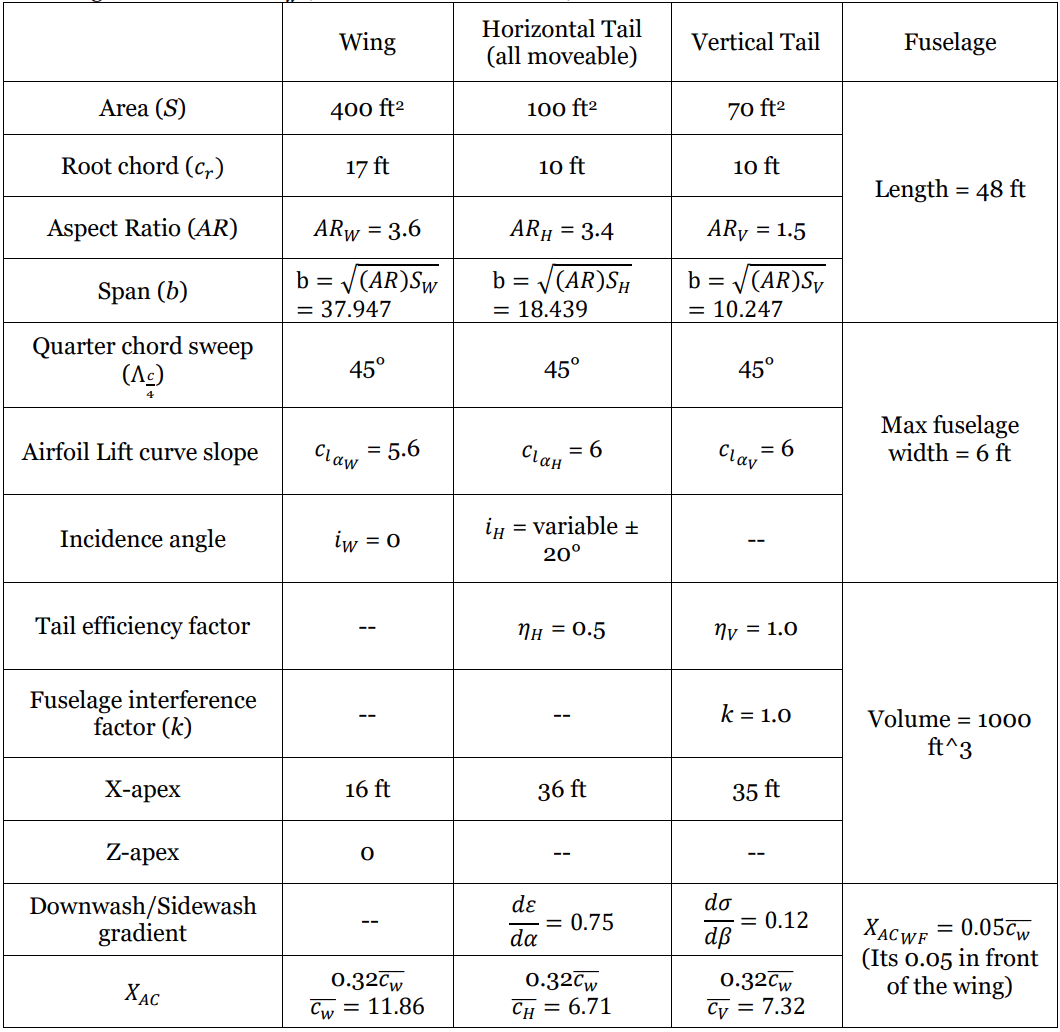
\includegraphics[width=\linewidth]{Givens-table.png}
\pagebreak
\begin{center}
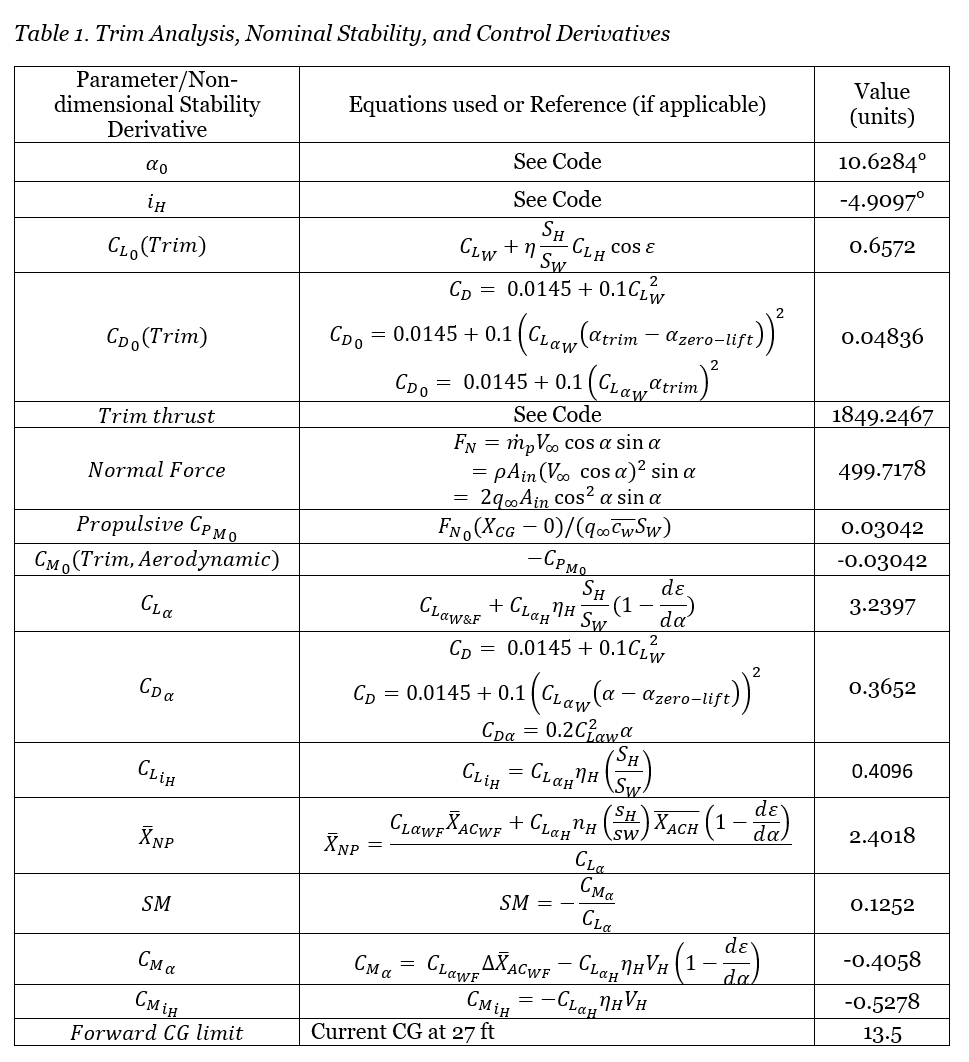
\includegraphics[width=\linewidth]{table-1.png}
\pagebreak
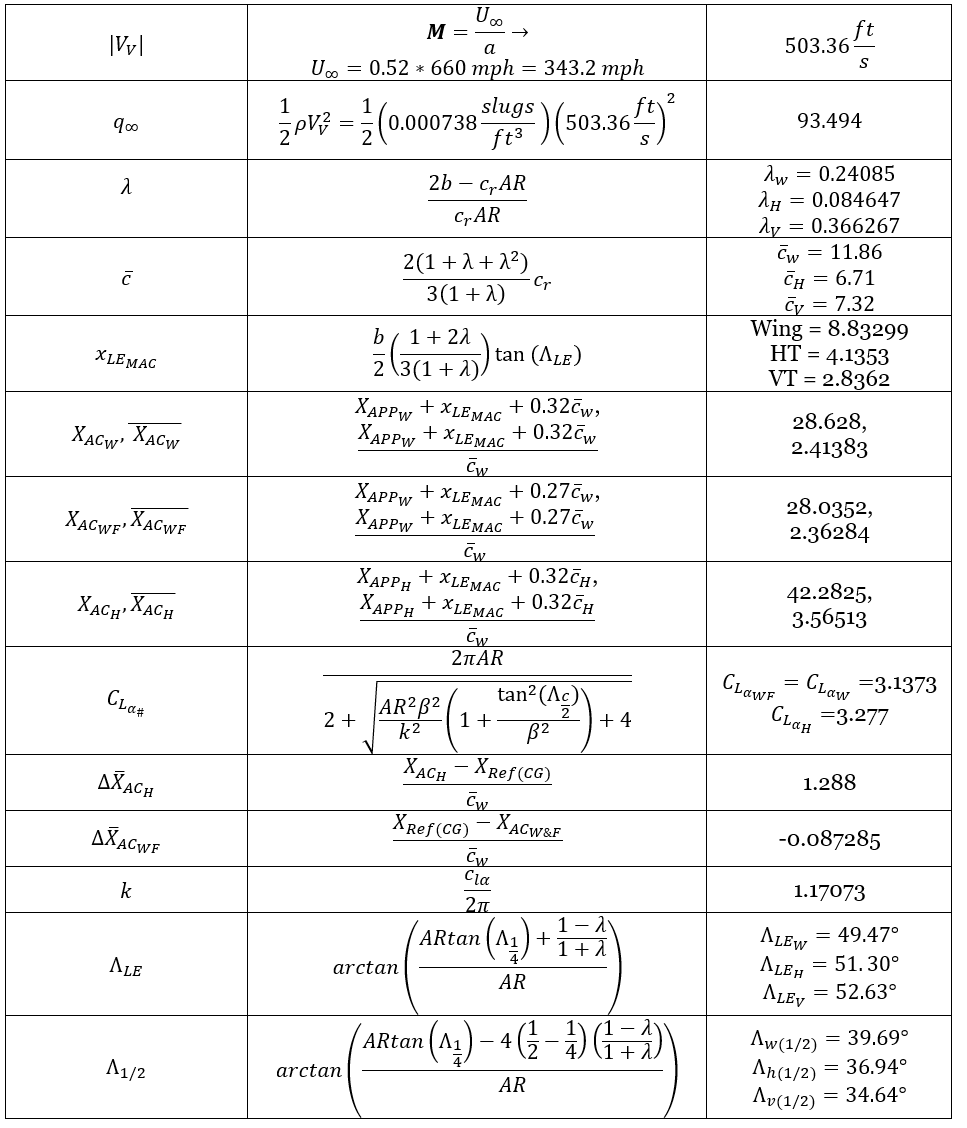
\includegraphics[width=\linewidth]{table-1-1.png}
\end{center}

\section{Task 2}

\subsection*{Summary of Longitudinal Stability and Control Derivatives}

\begin{enumerate}

\item \textbf{\(C_{D_M}\) and \(C_{L_M}\): Drag and Lift Contributions due to Pitching Motion}
\begin{align*}
C_{D_M} &= \frac{M \cos^2(q_{c_W})}{1 - M^2 \cos^2(q_{c_W})} \cdot C_{D0} \\
C_{L_M} &= \frac{M \cos^2(q_{c_W})}{1 - M^2 \cos^2(q_{c_W})} \cdot C_{L0}
\end{align*}

\item \textbf{\(C_{M_q}\): Pitch Damping Derivative}
\[
C_{M_q} = -n_H \cdot CL_{a_H} \cdot \frac{S_H}{S_W} \cdot (X_{ac_h} - X_{cg})^2 \cdot \cos^2(\alpha) \cdot \frac{1}{U_0 \cdot c_{w_w}}
\]

\item \textbf{\(C_{M_{\dot{a}}}\): Rate of Change of Pitch Damping with Respect to Angle of Attack}
\begin{equation*}
C_{M_{\dot{\alpha}}} = -n_H \cdot \frac{S_H}{S_W} \cdot CL_{a_H} \cdot (X_{ac_h} - X_{cg}) \cdot (X_{ac_h} - X_{ac_W}) \cdot \cos^2(\alpha) \cdot \delta_{e/\delta_{a}}
\end{equation*}

\item \textbf{\(X_u\), \(Z_u\), \(M_u\): Longitudinal Stability Derivatives}
\begin{align*}
X_u &= -\frac{(C_{D_u} + \frac{2}{U_0} \cdot C_{D0}) \cdot q_{\infty} \cdot S_W}{m} \\
Z_u &= -\frac{(C_{L_u} + \frac{2}{U_0} \cdot C_{L0}) \cdot q_{\infty} \cdot S_W}{m} \\
M_u &= -\frac{(C_{M_u} + \frac{2}{U_0} \cdot -\text{{prop\_CP\_M0}}) \cdot q_{\infty} \cdot S_W \cdot c_{w_w}}{I_{yy}}
\end{align*}

\item \textbf{\(X_a\), \(Z_a\), \(M_a\): Longitudinal Control Derivatives}
\begin{align*}
X_a &= -\frac{(-C_{D_{\alpha}} + C_{L0}) \cdot q_{\infty} \cdot S_W}{m} \\
Z_a &= -\frac{(-CL_{\alpha} + C_{D0}) \cdot q_{\infty} \cdot S_W}{m} \\
M_a &= \frac{C_{M_{\alpha}} \cdot q_{\infty} \cdot S_W \cdot c_{w_w}}{I_{yy}}
\end{align*}

\item \textbf{\(M_q\): Pitch Control Derivative}
\[
M_q = \frac{C_{M_q} \cdot q_{\infty} \cdot S_W \cdot c_{w_w}}{I_{yy}}
\]

\end{enumerate}


\pagebreak
\begin{center}
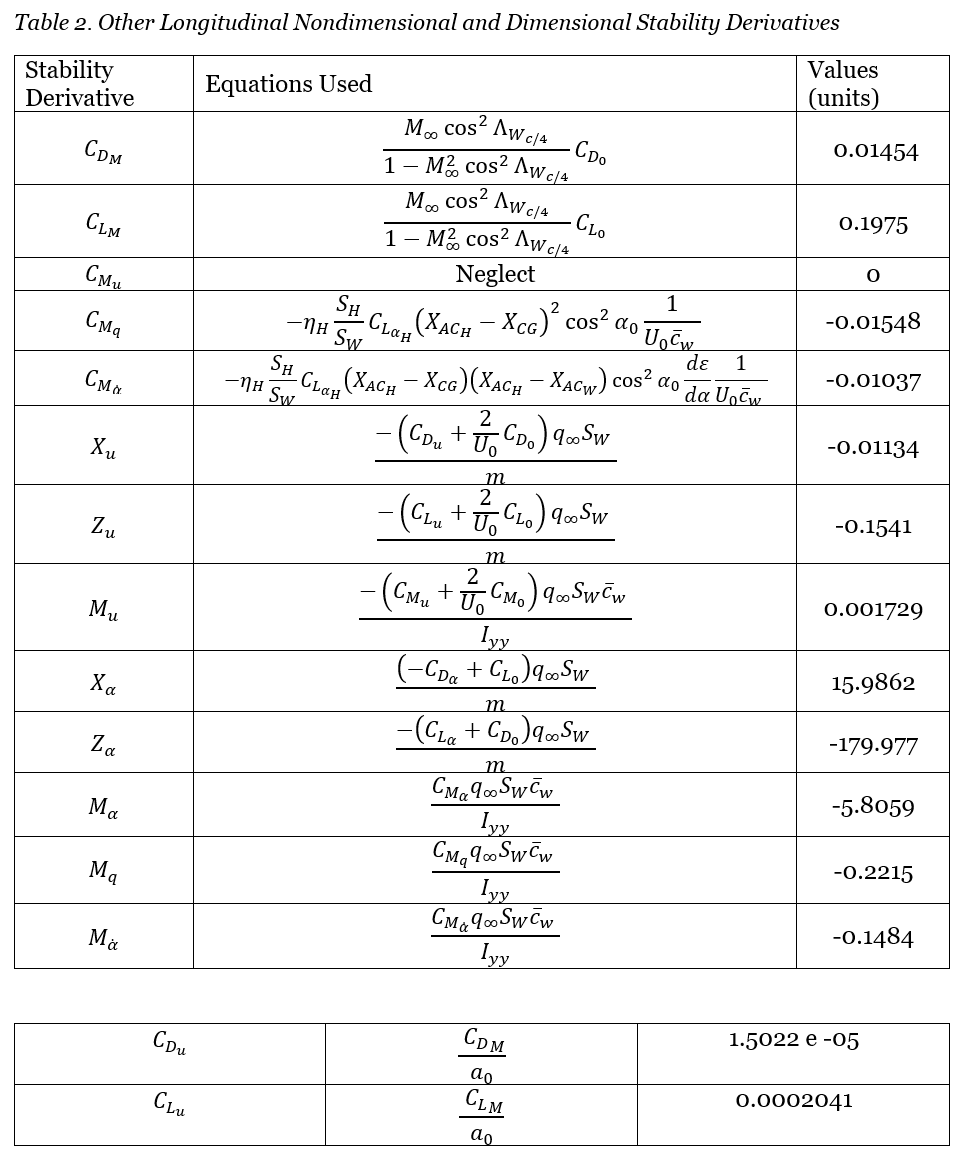
\includegraphics[width=\linewidth]{table-2.png}
\end{center}
\pagebreak
% \newpage
% \printbibliography
\subsection{Analysis of the Longitudinal Derivatives}

\[
\mathbf{A_{\text{mat}}} = \begin{bmatrix}
X_u & X_a & 0 & -32.2 \\
\frac{Z_u}{U_0} & \frac{Z_a}{U_0} & 1 & 0 \\
\frac{M_u + M_a\dot{Z_u}}{U_0} & \frac{M_a + M_a\dot{Z_a}}{U_0} & M_q + M_a\dot{Z_a} & 0 \\
0 & 0 & 1 & 0
\end{bmatrix}
\]


\begin{align*}
A &= \text{eig.real} \\
B &= \text{eig.imag} \\
\text{natural\_freq} &= \sqrt{A^2 + B^2} \\
\text{damping\_ratio} &= -\frac{A}{\text{natural\_freq}} \\
\text{time\_to\_half} &= \frac{\log{2}}{\left|A\right|} \\
\text{time\_constant} &= \frac{1}{\left|A\right|} \\
\text{cycle\_to\_half} &= \left|\frac{\text{time\_to\_half}}{2\pi / B}\right|
\end{align*}

\subsection{Explanation of Dynamic Parameters from Eigenvalues}

The eigenvalues of the longitudinal derivatives matrix provide valuable information about the dynamic behavior of the system. From these eigenvalues (\(A\) and \(B\)), several key parameters are derived:

\subsection*{Natural Frequency (\(\omega_n\))}

The natural frequency is determined from the real and imaginary parts of the eigenvalues using the formula:
\[ \text{natural\_freq} = \sqrt{A^2 + B^2} \]
It represents the rate at which the system oscillates without damping when disturbed.

\subsection*{Damping Ratio (\(\zeta\))}

The damping ratio is calculated as the negative ratio of the real part to the natural frequency:
\[ \text{damping\_ratio} = -\frac{A}{\text{natural\_freq}} \]
It provides information about the rate at which the system's amplitude decreases over time.

\subsection*{Time to Half Amplitude (\(t_{1/2}\))}

The time to half amplitude is computed as the natural logarithm of 2 divided by the absolute value of the real part of the eigenvalue:
\[ \text{time\_to\_half} = \frac{\log{2}}{\left|A\right|} \]
It indicates the time it takes for the system's amplitude to decrease to half of its initial value.

\subsection*{Time Constant (\(\tau\))}

The time constant is the reciprocal of the absolute value of the real part of the eigenvalue:
\[ \text{time\_constant} = \frac{1}{\left|A\right|} \]
It represents the time required for the system's response to reach \(1 - \frac{1}{e}\) (approximately 63.2%) of its final value.

\subsection*{Cycles-to-Half (\(n_{1/2}\))}

Cycles-to-half is calculated by taking the absolute value of the time to half amplitude and dividing it by the period of oscillation:
\[ \text{cycle\_to\_half} = \left|\frac{\text{time\_to\_half}}{2\pi / B}\right| \]
It gives the number of oscillations required for the system's amplitude to decrease to half.

These parameters provide insights into the dynamic behavior of the system, crucial for stability and control analysis in aerospace engineering.
\subsection{Categorzing the Aircraft}
By leveraging the content presented in the lecture slides, we gain the capability to systematically classify aircraft according 
to their performance and stability characteristics. 
The comprehensive insights provided in these educational materials allow us to analyze and categorize various aircraft models,
 taking into consideration factors such as aerodynamic performance, longitudinal and lateral stability, and other crucial parameters.
  This categorization is instrumental in enhancing our understanding of different aircraft types, 
  their design principles, and their operational capabilities, thereby contributing to a more profound comprehension of 
  aeronautical engineering principles and the broader field of aviation.


\subsection{Task 2 Tables}
\begin{center}
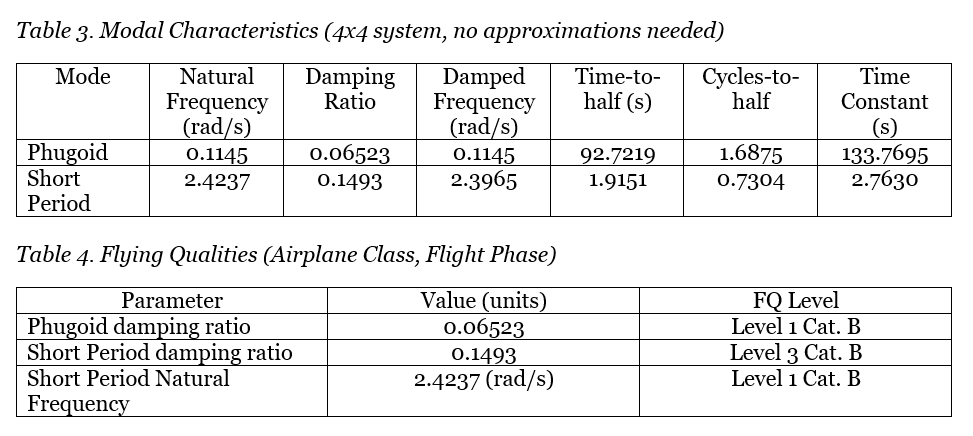
\includegraphics[width=\linewidth]{table-2-1.png}
\end{center}
\pagebreak

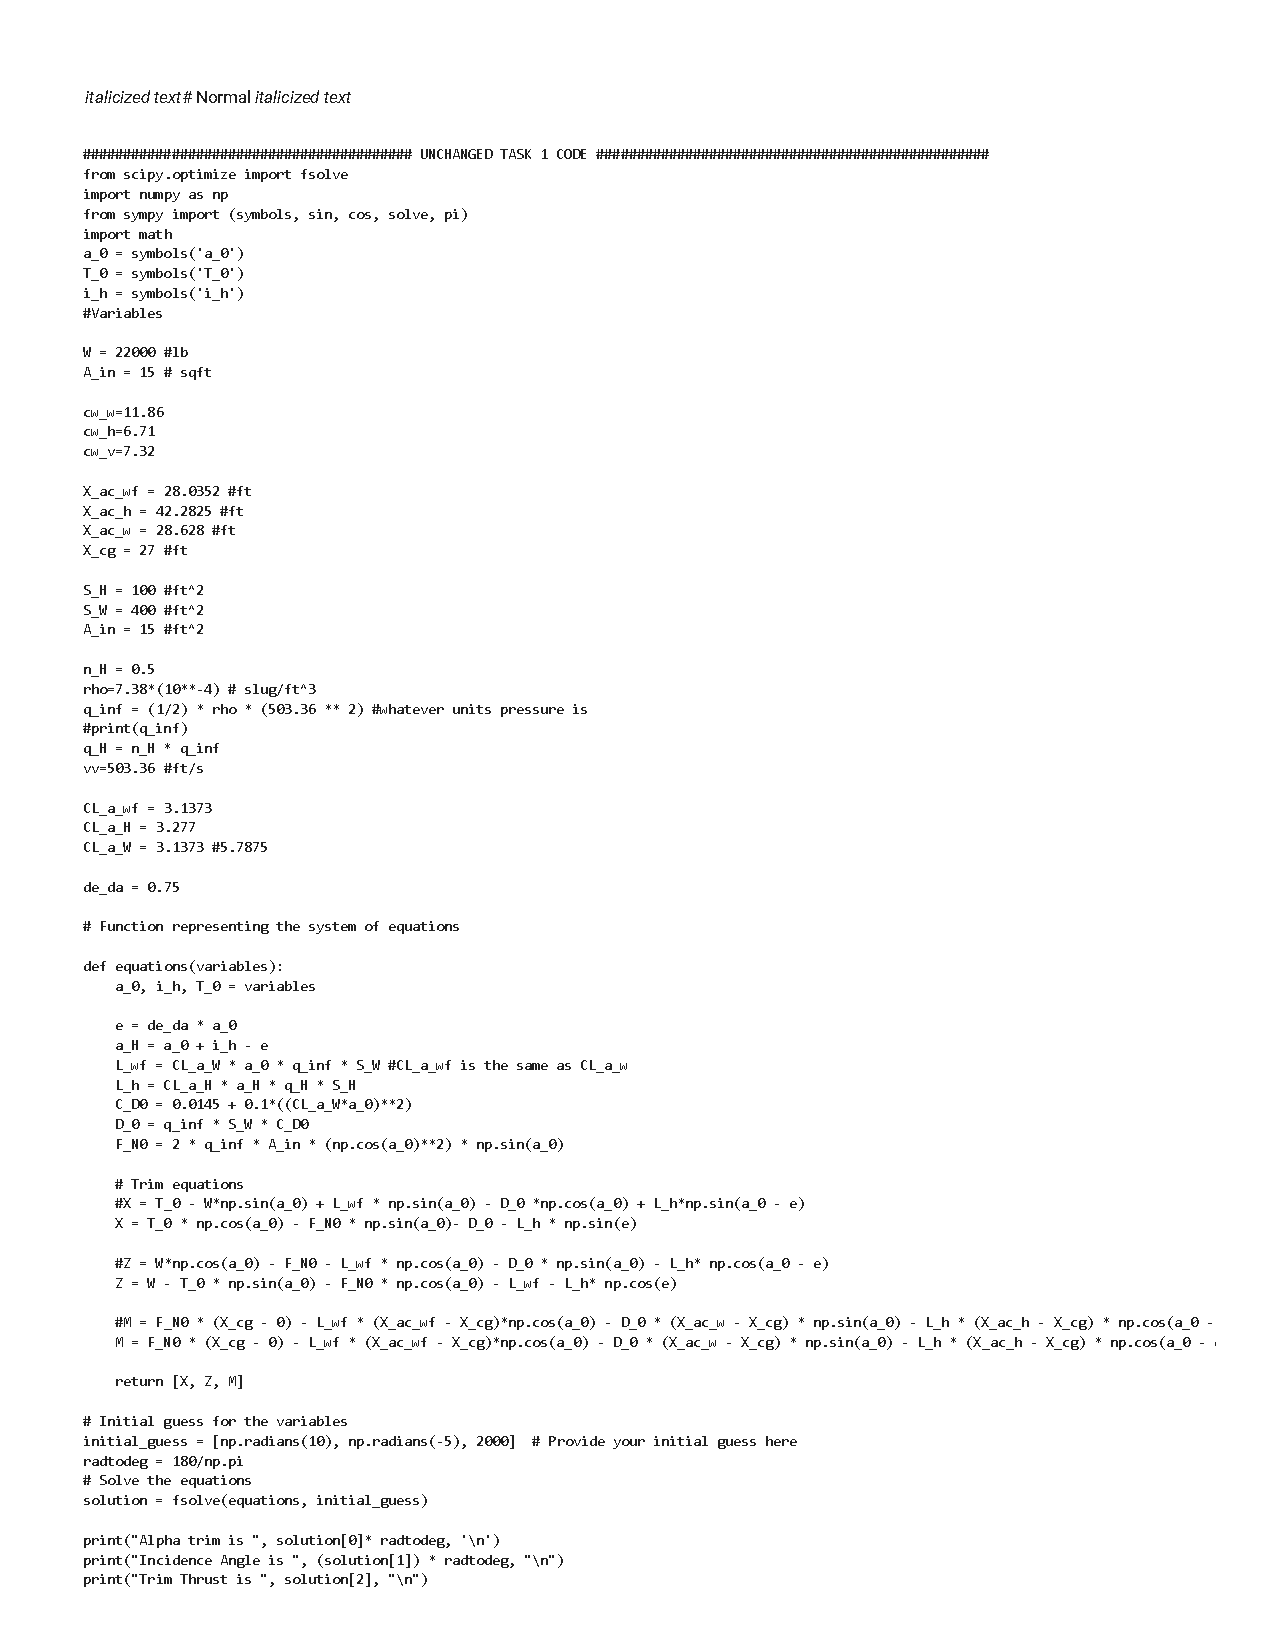
\includepdf[pages=-]{Code.pdf}
\end{document}